%!TEX root=paper/paper.tex
\begin{figure}[ht]
\centering
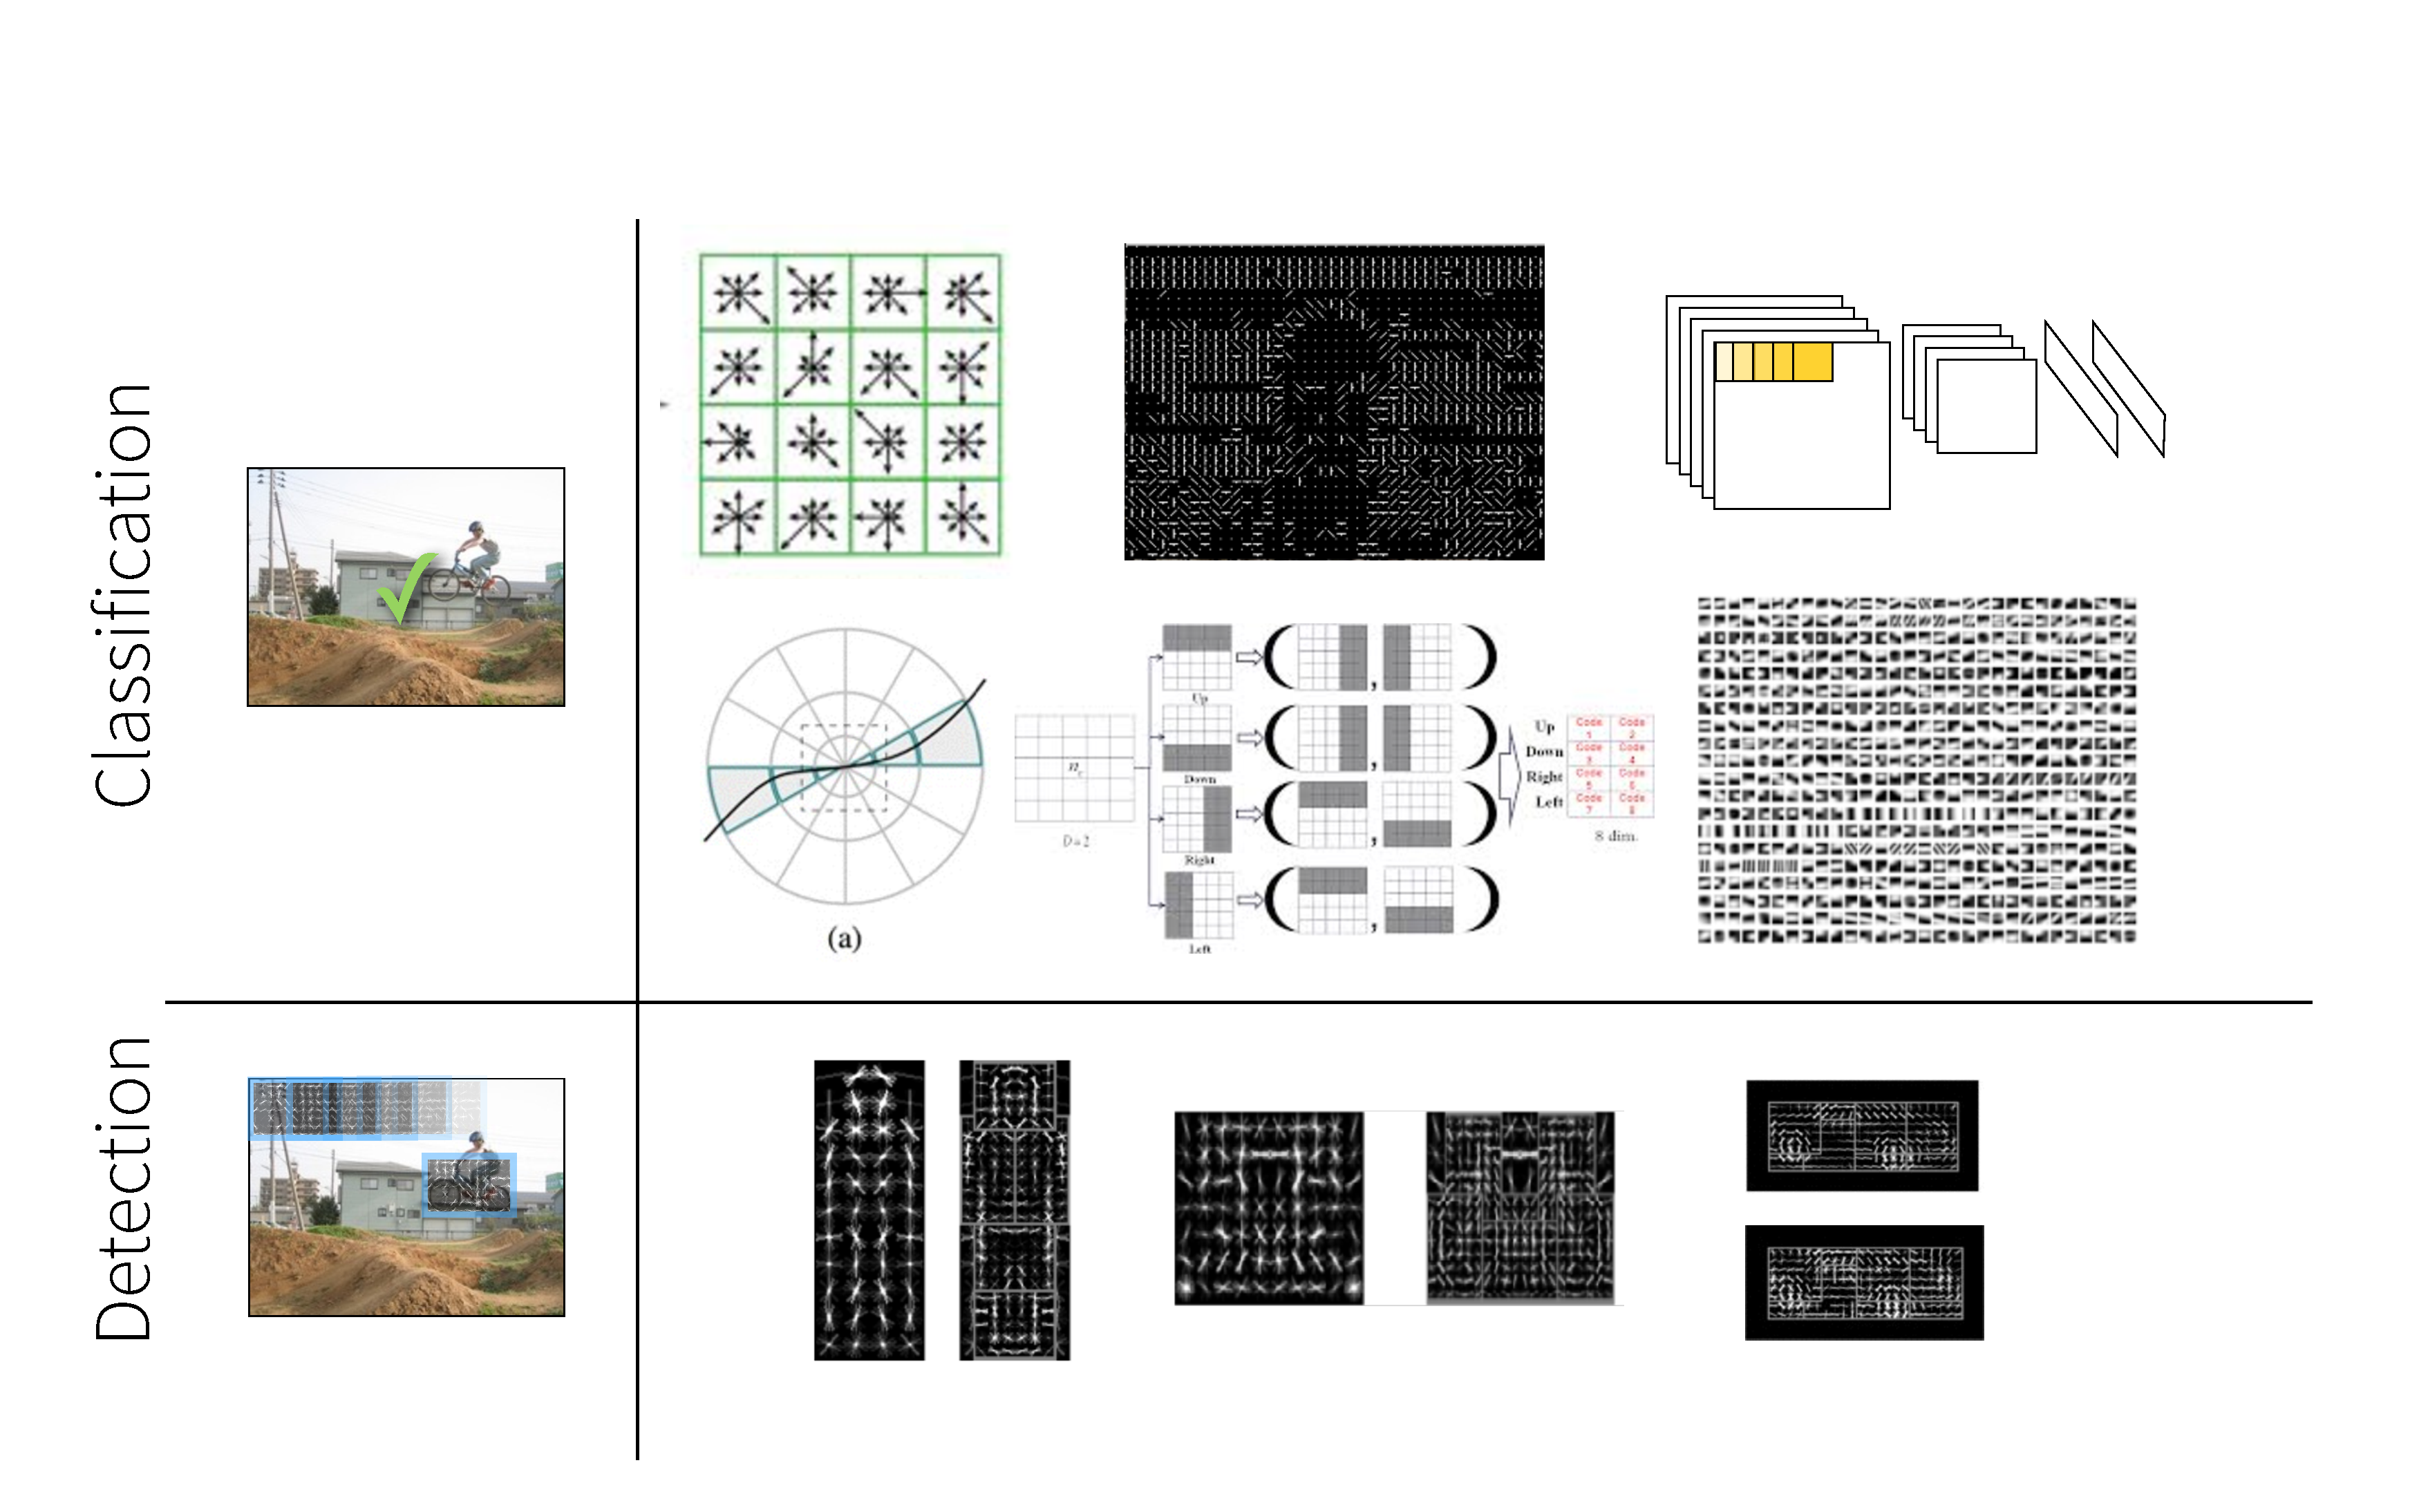
\includegraphics[width=\linewidth]{../../figures/features.pdf}
\caption[Summary of the variety of features for object detection and classification.]{
Summary of the variety of features for object detection and classification.
In reading order for classification: SIFT \parencite{Lowe2004}, HOG \parencite{Dalal2005}, CNN \parencite{Krizhevsky-NIPS-2012}, Self-Similarity \parencite{Shechtman2007}, Haar basis functions \parencite{Viola-IJCV-2004}, basis functions learned with sparse coding \parencite{Olshausen1996}.
In reading order for detection: person, bicycle, and car templates for the Deformable Part Model \parencite{Felzenszwalb2010a}.
(The features depicted were not computed on the images depicted.)
}\label{fig:features}
\end{figure}
